\documentclass[a4paper,10pt]{article}
\addtolength{\textwidth}{5.2cm}
\addtolength{\voffset}{-3cm}
\addtolength{\hoffset}{-2.5cm}
\addtolength{\textheight}{5cm}
\addtolength{\headheight}{14.0pt}
\usepackage[utf8]{inputenc}
\usepackage[spanish,activeacute]{babel} 
\usepackage{paralist}
\usepackage[pdftex]{graphicx}
\usepackage{epsfig}
% \usepackage[T1]{fontenc}
% \usepackage{cmap}
% \usepackage{fix-cm}
% \usepackage{lscape}
% \usepackage{amsmath}
% \usepackage{amssymb}
% \usepackage{mathrsfs}
% \usepackage{epstopdf}
% % \usepackage{algorithmic}
\usepackage{verbatim}
% \usepackage[lined,boxed,commentsnumbered]{algorithm2e}
% \usepackage{graphicx}
% \usepackage[utf8]{inputenc}
\usepackage{lscape}

\usepackage{caratulayabs} %Para la caratula
\usepackage[pdfborder={0,0,0}]{hyperref}
% \usepackage{ifthen}
% \usepackage{paralist}
% \usepackage{ulem}

\newcommand{\dotu}{\bgroup \markoverwith{\lower .4ex\hbox{\_}}\ULon} % para subrallado punteados

\newcommand{\header}[1]{\textsf{#1}}
\newcommand{\todo}[1]{\frame{\textsf{TODO} #1}}

%Redefino algunos nombres (como uso babel, lo tengo que hacer asi):
% Donde dice \chapter quiero que aparezca Problema en lugar de Capitulo
\addto\captionsspanish{% esto lo necesito porque uso babel
  \renewcommand{\chaptername}%
    {Cap\'itulo}%
}

%Donde dice Indice general, quiero que aparezca Contenidos
\addto\captionsspanish{% esto lo necesito porque uso babel
  \renewcommand{\contentsname}%
    {Contenidos}%
}

%Donde dice Indice general, quiero que aparezca Contenidos
\addto\captionsspanish{% esto lo necesito porque uso babel
  \renewcommand{\appendixname}%
    {Anexo}%
}

%Donde dice Cuadro, quiero que aparezca Tabla
\addto\captionsspanish{% esto lo necesito porque uso babel
  \renewcommand{\tablename}%
    {Tabla}%
}

\DeclareMathAlphabet{\mathpzc}{OT1}{pzc}{m}{it}

\input ulem.sty

\usepackage{tikz}

\newcommand{\udot}[1]{%
    \tikz[baseline=(todotted.base)]{
        \node[inner sep=1pt,outer sep=0pt] (todotted) {#1};
        \draw[dotted] (todotted.south west) -- (todotted.south east);
    }%
}%


\newcommand{\uloosdash}[1]{%
    \tikz[baseline=(todotted.base)]{
        \node[inner sep=1pt,outer sep=0pt] (todotted) {#1};
        \draw[loosely dashed] (todotted.south west) -- (todotted.south east);
    }%
}%
\newcommand{\udash}[1]{%
    \tikz[baseline=(todotted.base)]{
        \node[inner sep=1pt,outer sep=0pt] (todotted) {#1};
        \draw[dashed] (todotted.south west) -- (todotted.south east);
    }%
}%

\newcommand{\udensdash}[1]{%
    \tikz[baseline=(todotted.base)]{
        \node[inner sep=1pt,outer sep=0pt] (todotted) {#1};
        \draw[densely dashed] (todotted.south west) -- (todotted.south east);
    }%
}%




\begin{document}



	% begin caratula
		\materia{Bases de datos}
		\submateria{Primer Cuatrimestre de 2013}
		\titulo{Trabajo Práctico 1}
		\subtitulo{Primera parte}
		\integrante{Mauricio Alfonso}{065/09}{mauricio.alfonso.88@gmail.com}
		\integrante{Ángel Abregú}{082/09}{angelj\_a@hotmail.com}
		\integrante{Esteban Capillo}{484/04}{estebancapillo@gmail.com}
		\integrante{Martín Rados}{185/93}{radosm@gmail.com}
		
		\maketitle
	% fin caratula

\newpage
\thispagestyle{empty}
\mbox{}

% indice:
	
% \tableofcontents

\newpage
\newpage

\section{Introducci\'on}
 
 En la actualidad, los clientes de una línea aérea pueden realizar reservas de pasajes desde su casa o el trabajo, si cuentan con un browser y una conexión a Internet.\\
 
Hoy en día todas las líneas aéreas tienen su sitio en la Web donde implementan su WIS (\textit{Web-based Information System}). Estos sistemas tienen en el Back-End un servidor Web que utiliza los servicios de un motor de base de datos.
En la mayoría de los casos el WIS no sólo permite reservar pasajes sino que además brinda una serie de servicios adicionales al viajero.\\
\\

En este trabajo se pretende diseñar e implementar una base de datos que brinde soporte al WIS de
una línea aérea hipotética.\\

Asumiremos que se implementará el WIS desde cero, o sea que no consideraremos los problemas
vinculados al pasaje y conversión de los datos y estructuras de los legacy system existentes.\\

El sistema deberá dar a los clientes usuarios la posibilidad de abrir una cuenta personal y registrar
sus datos y preferencias, reservar pasajes y hacer consultas varias.
\\

Los servicios que deberá brindar el WIS al cliente (en el Front-End) son los
siguientes:
\begin{itemize}
\item Abrir una cuenta con información personal y preferencias de viaje
\item Consultar disponibilidad de vuelos
\item Consultar tarifas
\item Armar un plan de viaje
\item Reservar pasajes
\item Consultar reservas efectuadas
\item Cancelar reservas
\end{itemize}

 
 Además, en el Back-End, deberá permitir a la compañía obtener informes de las operaciones llevadas a
cabo por sus clientes. Las funcionalidades que deben implementarse se detallan en una sección al final de este informe.


 \newpage

\section{Modelos}

\subsection{Modelo Entidad-Relaci\'on}

% \begin{landscape}
% 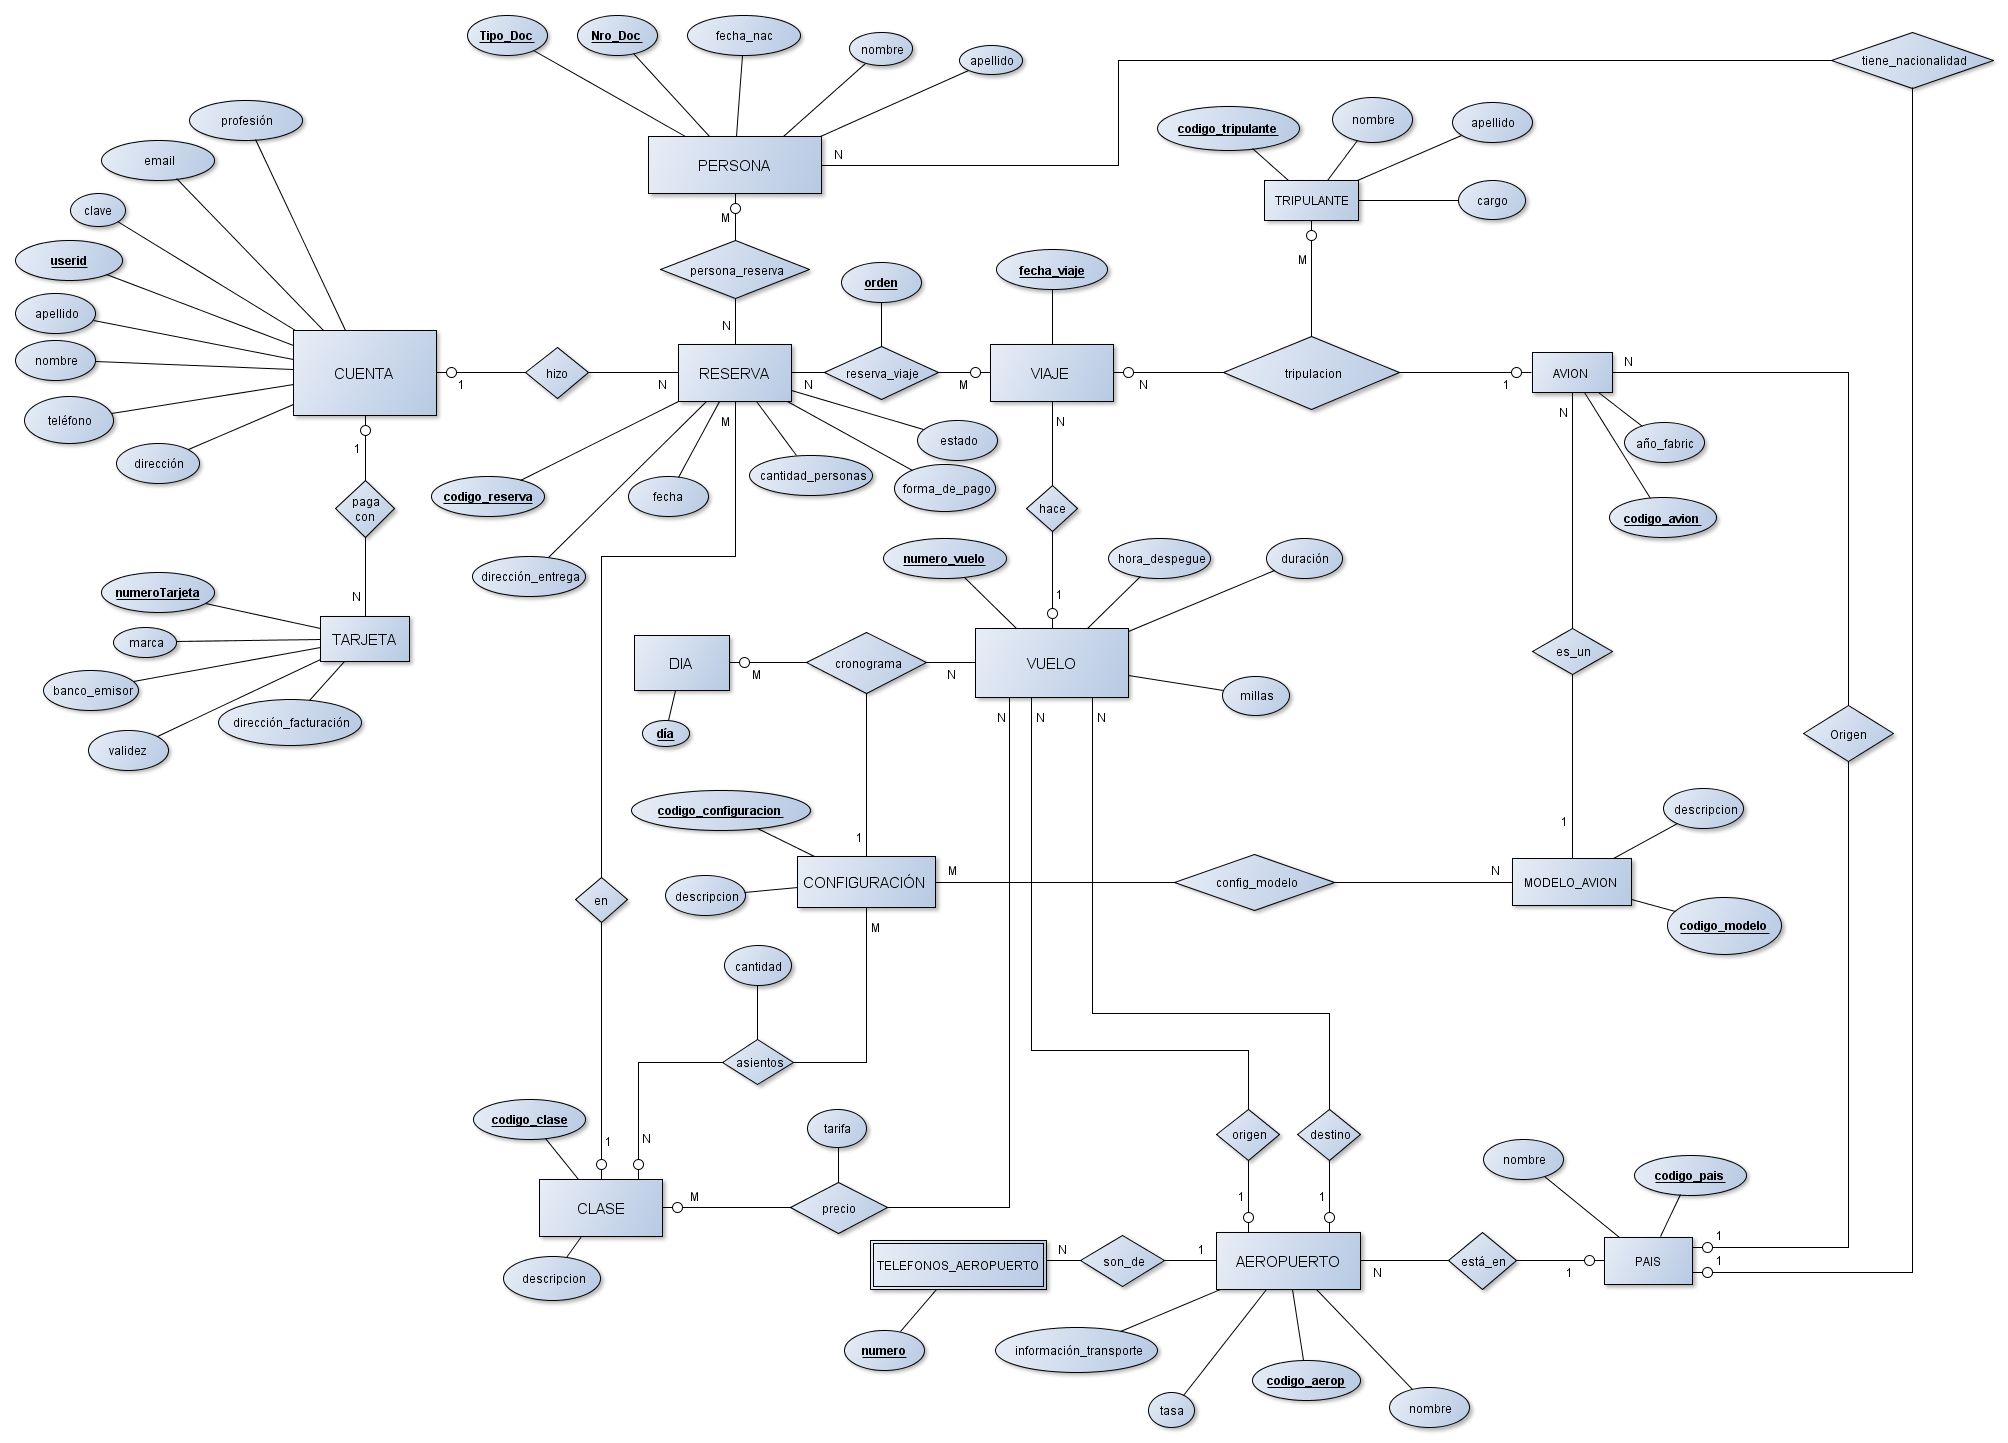
\includegraphics[scale=.35]{DER.png}
% \end{landscape}

% \begin{figure}[!h]
% \centering
% 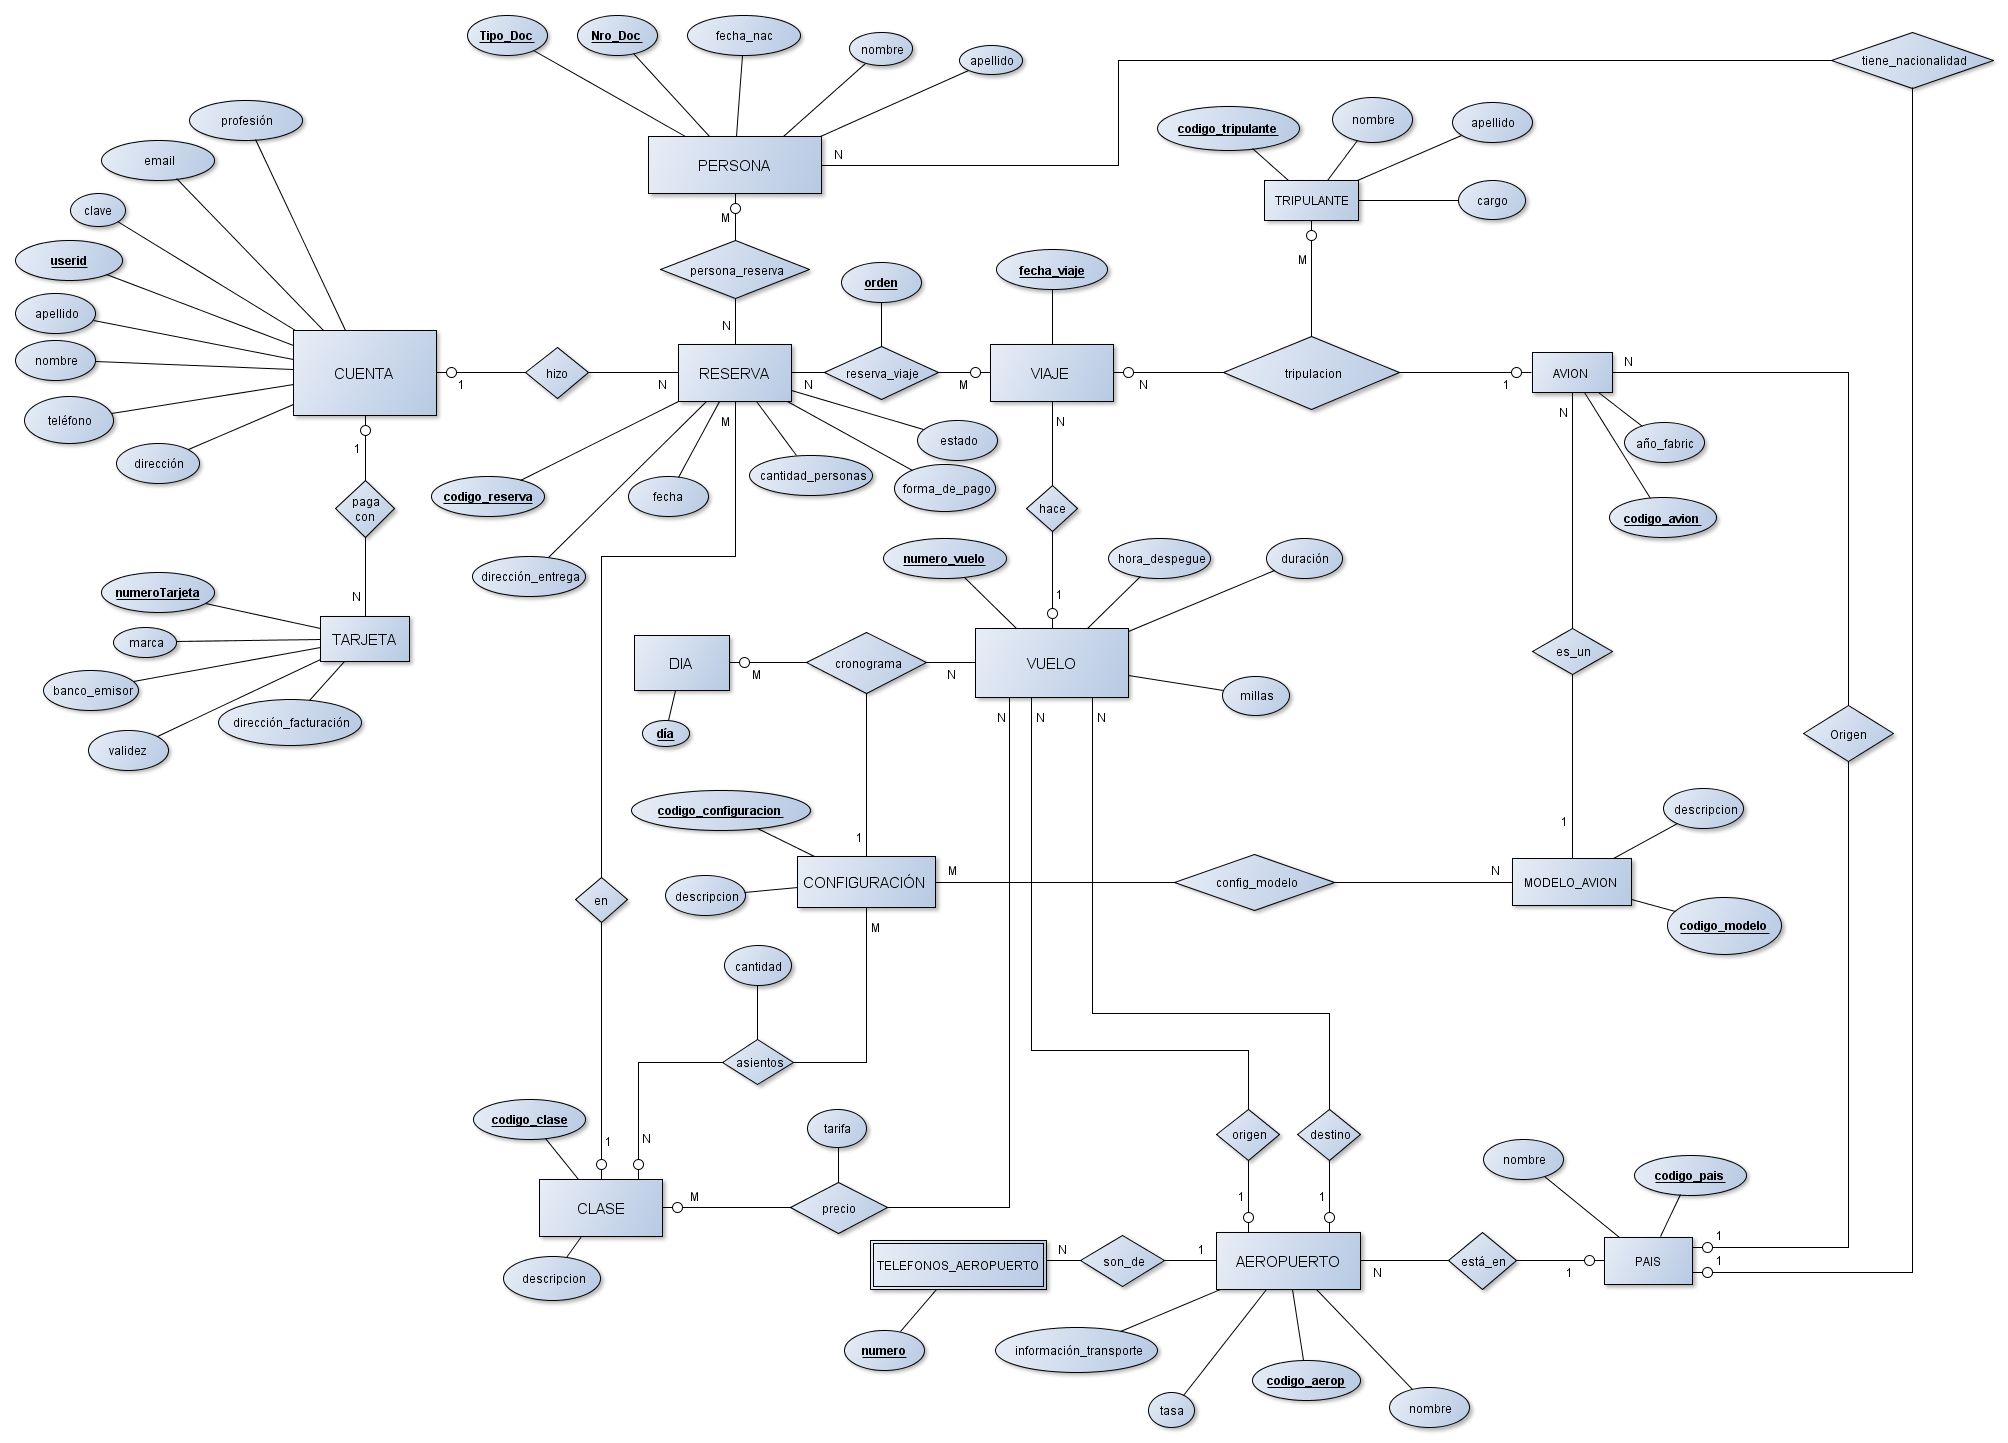
\epsfig{file=./DER.png,width=0.9\linewidth,clip=}
% % \caption{Análisis de rendimiento de los scans con respecto a la cantidad de puertos scanneados.}
% \end{figure}

\begin{figure}[h!]
\centering
    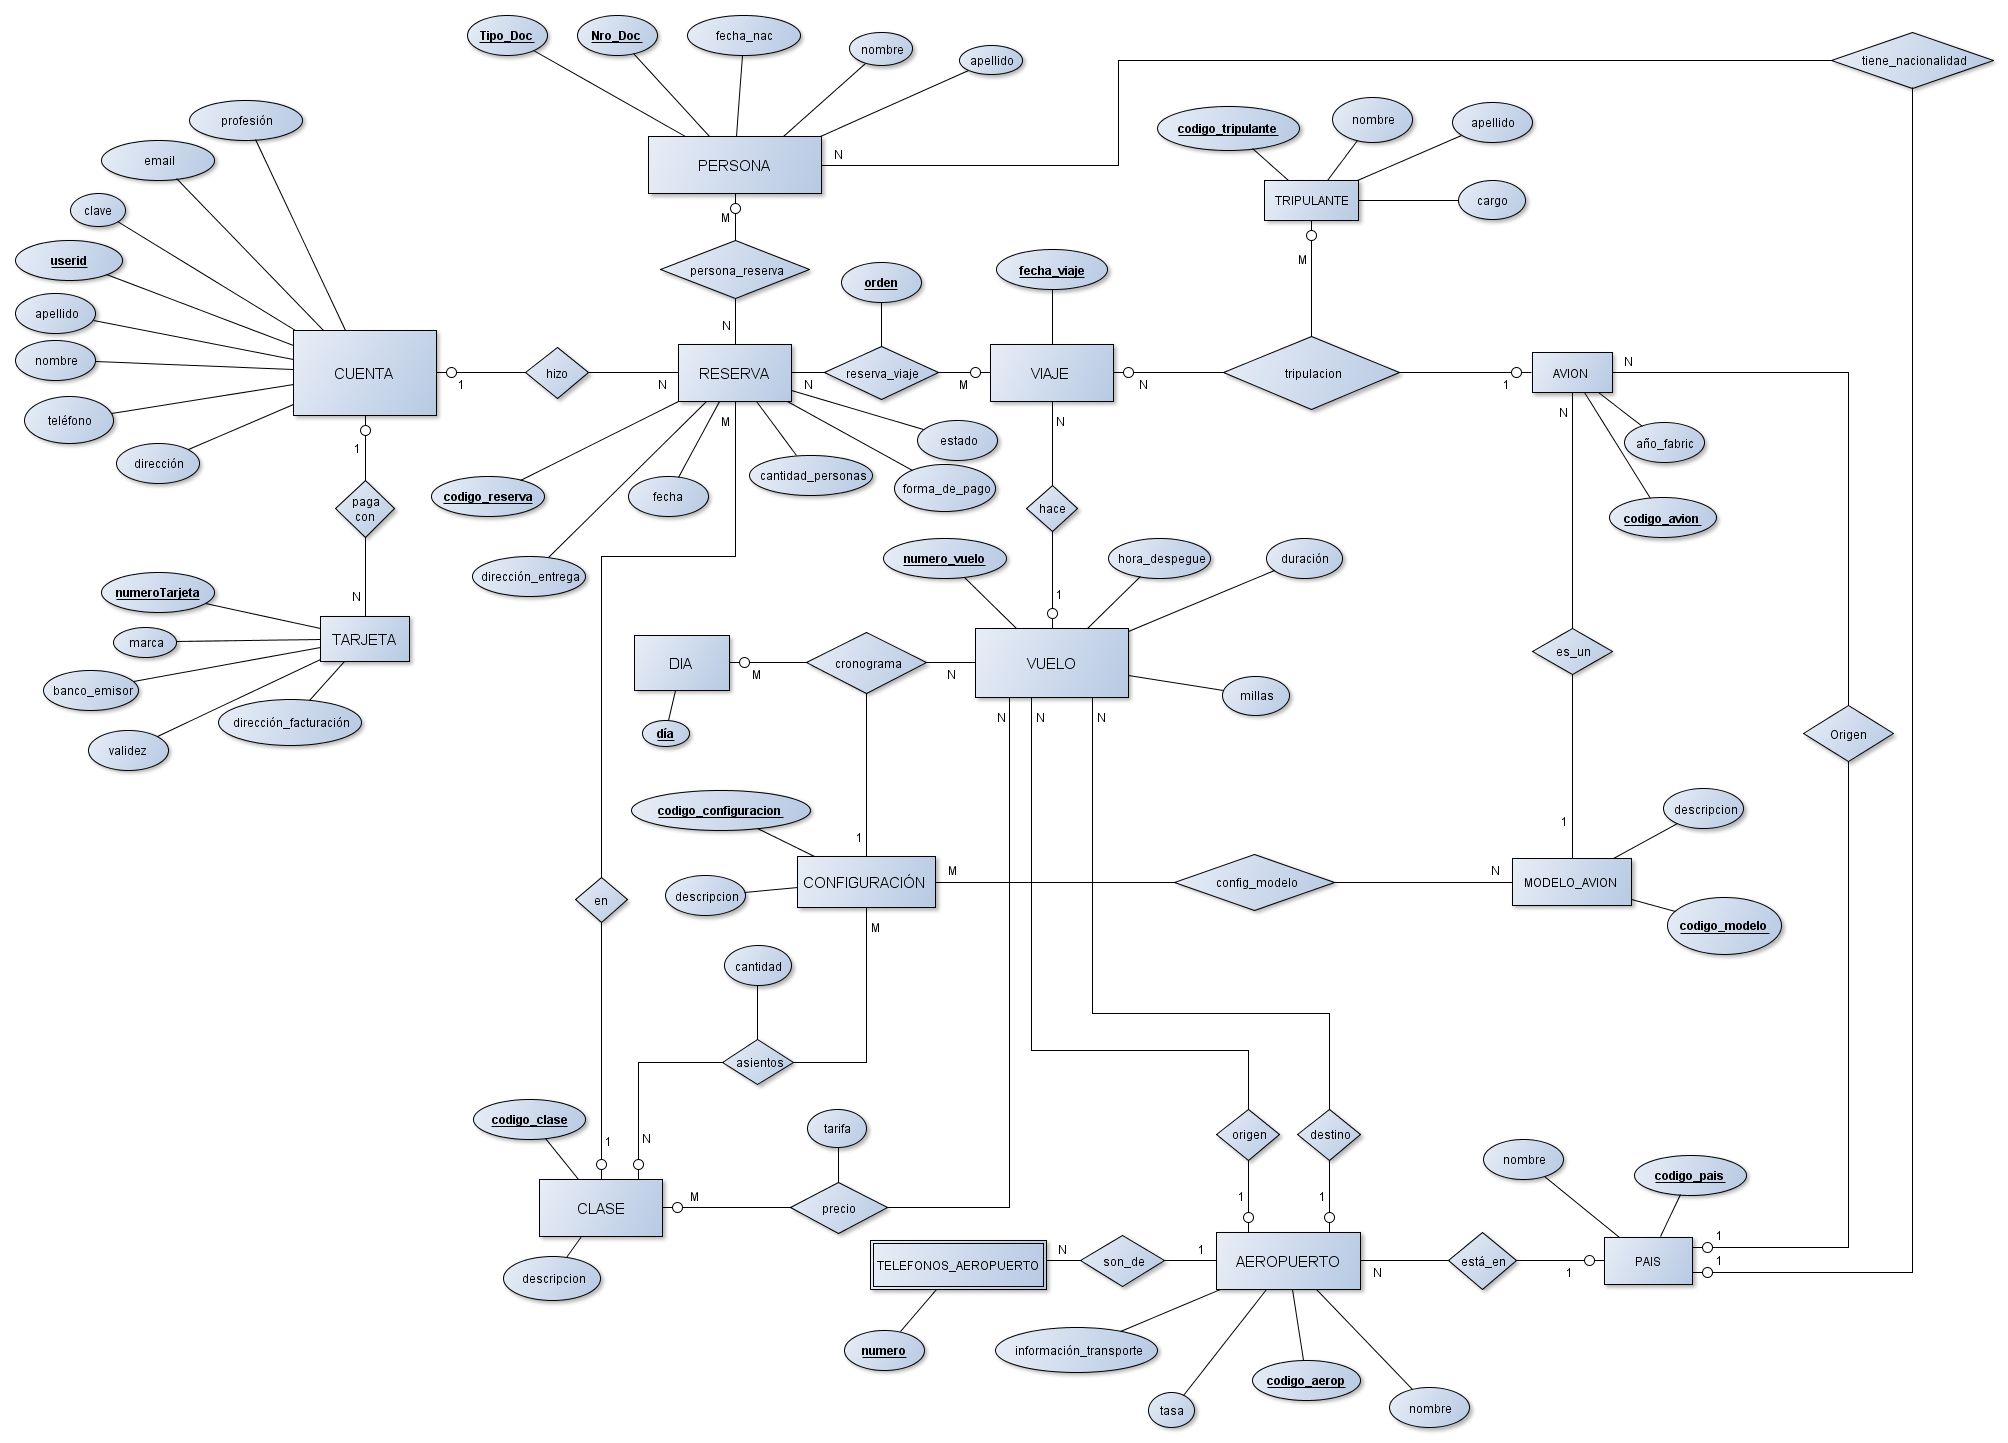
\includegraphics[angle=90, scale=.33]{DER.png}
\end{figure}


\subsection{Modelo Relacional}

\begin{itemize}
  \item \texttt{Cuenta(profesión, email, clave, \underline{userid}, apellido, nombre, teléfono, dirección)
  \\ \\PK = CK = \{userid\}
  \\FK = \{\} 
  }

  \item \texttt{Tarjeta(\udash{userid}, \underline{numeroTarjeta}, marca, banco\_emisor, validez, dirección\_facturación)
  \\ \\PK = CK = \{numeroTarjeta\}
  \\FK = \{userid\}
  }

  \item \texttt{Reserva(\udash{userid, codigo\_clase}, \underline{codigo\_reserva}, dirección\_entrega, fecha, forma\_de\_pago, estado, cantidad\_personas)
  \\ \\PK = CK = \{codigo\_reserva\}
  \\FK = \{userid, codigo\_clase\} 
  }

  \item \texttt{persona\_reserva(\underline{\udash{tipo\_doc, nro\_doc, codigo\_reserva}})
  \\ \\PK = CK = FK = \{(tipo\_doc, nro\_doc, codigo\_reserva)\}
  }

  \item \texttt{Persona(\underline{tipo\_doc, nro\_doc}, fecha\_nac, \dotu{codigo\_pais}, nombre, apellido)
  \\ \\PK = CK = \{(tipo\_doc, nro\_doc)\}
  \\FK = \{codigo\_pais\}
  }

  \item \texttt{reserva\_viaje(\underline{orden, \udash{codigo\_reserva, numero\_vuelo, fecha\_viaje}})
  \\ \\PK = CK = \{(orden, codigo\_reserva, numero\_vuelo, fecha\_viaje)\}
  \\FK = \{codigo\_reserva, numero\_vuelo, fecha\_viaje\}}

  \item \texttt{Viaje(\underline{fecha\_viaje, \udash{numero\_vuelo}})
  \\ \\PK = CK = \{(fecha\_viaje, numero\_vuelo)\}
  \\FK = \{numero\_vuelo\}}

  \item \texttt{Vuelo(\underline{numero\_vuelo}, hora\_despegue, duración, millas, \udash{origen, destino})
  \\ \\PK = CK = \{numero\_vuelo\}
  \\FK = \{origen, destino\}}

  \item \texttt{cronograma(\underline{\udash{día, numero\_vuelo}}, \udash{codigo\_configuracion})
  \\ \\PK = CK = \{(día, número\_vuelo)\}
  \\FK = \{día, numero\_vuelo, codigo\_configuracion\}}

  \item \texttt{Dia(\underline{día})
  \\ \\PK = CK = \{día\}
  \\FK = \{\}}

  \item \texttt{Configuración(\underline{codigo\_configuración}, descripción)
  \\ \\PK = CK = \{codigo\_configuración\}
  \\FK = \{\}}

  \item \texttt{asientos(\underline{\udash{codigo\_configuracion, codigo\_clase}}, cantidad)
  \\ \\PK = CK = FK = \{(codigo\_configuracion, codigo\_clase)\}}

  \item \texttt{Clase(\underline{codigo\_clase}, descripción)
  \\ \\CK = \{codigo\_clase, descripcion\}
  \\PK = \{codigo\_clase\}
  \\FK = \{\}}

  \item \texttt{Precio(\underline{\udash{numero\_vuelo, codigo\_clase}}, tarifa)
  \\ \\PK = CK = FK = \{numero\_vuelo, codigo\_clase\}}

  \item \texttt{config\_modelo(\underline{\udash{codigo\_configuracion, codigo\_modelo}})
  \\ \\PK = CK = FK = \{codigo\_configuracion, codigo\_modelo\}}

  \item \texttt{Modelo\_avion(\underline{codigo\_modelo}, descripcion)
  \\ \\PK = CK = \{codigo\_modelo\}
  \\FK = \{\}}

  \item \texttt{Avion(\underline{codigo\_avion}, año\_fabric, \udash{codigo\_modelo, codigo\_pais})
  \\ \\PK = CK = \{codigo\_avion\}
  \\FK = \{codigo\_modelo, codigo\_pais\}}
  
  \item \texttt{tripulacion(\underline{\udash{fecha\_viaje, numero\_vuelo, codigo\_tripulante}}, \udash{codigo\_avion})
  \\ \\PK = CK = \{(fecha\_viaje, numero\_vuelo, codigo\_tripulante)\}
  \\FK = \{fecha\_viaje, numero\_vuelo, codigo\_tripulante, codigo\_avion\}}

  \item \texttt{Tripulante(\underline{codigo\_tripulante}, nombre, apellido, cargo)
  \\ \\PK = CK = \{codigo\_tripulante\}
  \\FK = \{\}}

  \item \texttt{Pais(\underline{codigo\_pais}, nombre)
  \\ \\CK = \{codigo\_pais, nombre\}
  \\ PK = \{codigo\_pais\}
  \\FK = \{\}}

  \item \texttt{Aeropuerto(\underline{codigo\_aeropuerto}, información\_transporte, tasa, nombre, \udash{codigo\_pais})
  \\ \\CK = \{codigo\_aerop, nombre\}
  \\ PK = \{codigo\_aerop\}
  \\FK = \{codigo\_pais\}}

  \item \texttt{Telefonos\_aeropuerto(\underline{numero, \udash{codigo\_aeropuerto}})
  \\ \\PK = CK = \{(numero, codigo\_aeropuerto\}
  \\FK = \{codigo\_aeropuerto\}}

\end{itemize}

\newpage

\subsection{Supuestos asumidos}

\begin{itemize}
 \item Denominamos \texttt{Vuelo} a un vuelo que se hace frecuentemente entre dos aeropuertos. \texttt{Viaje} es una instancia particular de \texttt{Vuelo}, es decir, un vuelo en una fecha en particular. Si una persona hace un viaje con escalas, entonces decimos que en realidad hace varios viajes, uno por cada tramo. Dichos viajes son agrupados en una \texttt{Reserva}, y el orden de los tramos est\'a indicado por el atributo \texttt{orden} de la relaci\'on \texttt{reserva\_viaje}.

  \item Una \texttt{Reserva} es para varias personas, pero asumimos que viajan en la misma clase. De la misma manera asumimos que todos los vuelos de una reserva son en la misma clase.

  \item Un \texttt{Vuelo} se hace varias al menos una vez por semana, siempre en el mismo horario. Asumimos que el mismo vuelo no se puede realizar dos veces en un mismo día. Denominamos \texttt{Configuración} a una manera de organizar los asientos por clase en un avión. Un vuelo puede tener varias configuraciones diferentes dependiendo del día de semana.
    
  \item El usuario que realiza una reserva debe garantizar que la combinación de viajes sea realizable según el \underline{\textbf{orden}} dado. Es decir, asumimos que para todo viaje $v$ de una misma reserva, el siguiente en orden (si existe) tiene que partir tiempo después que $v$ llegue, y además, el aeropuerto de origen ser el aeropuerto de llegada de $v$.
  
\end{itemize}

\subsection{Restricciones adicionales}

\begin{itemize}

  \item Las fechas de los viajes son tales que el vuelo correspondiente tenga un cronograma en ese día.

  \item Para todo viaje y toda clase, la cantidad de asientos del vuelo correspondiente en esa clase en el día de semana correspondiente al de la fecha del viaje, debe ser mayor o igual a la cantidad de personas con reservas de ese viaje en esa clase.

  \item Las clases de todas las configuraciones de un vuelo deben ser las mismas que las clases de los precios de ese vuelo.

  \item El avión de un viaje tiene un modelo que cumple con la configuración de asientos correspondiente al vuelo y día de ese viaje.

  \item El aeropuerto de origen de un vuelo es distinto del aeropuerto de destino.

\end{itemize}

\newpage
\section{Funcionalidades}

% hay que reemplazar todos los tabs por espacios para que quede bien

\subsection{Consulta de pasajeros}

FALTA EXPLICACION

\begin{verbatim}

\end{verbatim}


\subsection{Reporte de aeropuertos}

La siguiente consulta realiza un reporte con los aeropuertos (identificados por sus códigos), para cada período \textit{Año/Mes} la cantidad de personas que subieron y que bajaron de ese aeropuerto,
dentro de un rango de fechas específico.

\begin{verbatim}
 
DROP VIEW IF EXISTS vw_paso_por;

--
-- reservas confirmadas, origen y destino
--
CREATE OR REPLACE VIEW vw_paso_por AS
  SELECT r.codigo_reserva,
    rv.fecha_viaje+v.hora_despegue salio, v.aeropuerto_ori,
    rv.fecha_viaje+v.hora_despegue+v.duracion llego, v.aeropuerto_dst
  FROM reserva r, reserva_viaje rv, vuelo v
  WHERE rv.codigo_reserva = r.codigo_reserva
  AND v.numero_vuelo=rv.numero_vuelo
  AND r.estado='confirmado';

--
-- Personas que subieron/bajaron de cada aeropuerto
--

SELECT aeropuerto, to_char(fecha, 'YYYY/Mon') periodo, sum(subio) subieron, sum(bajo) bajaron 
FROM (
  SELECT pp.aeropuerto_ori aeropuerto, pp.salio fecha, cantidad_personas subio, 0 bajo
  FROM vw_paso_por pp,
     (SELECT codigo_reserva, count(*) cantidad_personas
      FROM persona_reserva GROUP BY codigo_reserva) pr
  WHERE pr.codigo_reserva = pp.codigo_reserva
  UNION ALL
  SELECT pp.aeropuerto_dst, pp.llego, 0, cantidad_personas
  FROM vw_paso_por pp,
     (SELECT codigo_reserva,count(*) cantidad_personas
      FROM persona_reserva GROUP BY codigo_reserva) pr
  WHERE pr.codigo_reserva = pp.codigo_reserva
) datos
WHERE fecha BETWEEN 'January 1, 2012' AND 'January 31, 2014'
GROUP BY aeropuerto,to_char(fecha, 'YYYY/Mon')
ORDER BY sum(subio)+sum(bajo) DESC, sum(subio) DESC;

\end{verbatim}

Hemos utilizado una \textit{vista} por razones de legibilidad, pero puede escribirse una consulta con equivalente sin hacer uso de ella.


\subsection{Trigger de reservas}

FALTA EXPLICACION

\begin{verbatim}
 

\end{verbatim}


\newpage
% \section{Conclusiones}
% 
% (falta)

\end{document}
